\section{Pruebas y Resultados}

%\subsection{Pruebas en ambiente controlado}
\begin{frame}{Pruebas en ambiente controlado}
\begin{block}{Caso ideal, conexión directa}
	\begin{itemize}
		%\subsection{ISDB-T (International Standard for Digital Broadcasting - Terrestrial)}	
		\item { Se decodificaron las tres capas exitosamente }
		\item { Verificamos la funcionalidad básica del sistema }
	\end{itemize}
\end{block}

\begin{block}{Caso ruidoso, simulamos perdidas en el canal}
	\begin{itemize}
		%\subsection{ISDB-T (International Standard for Digital Broadcasting - Terrestrial)}	
		\item {	Observamos el efecto de los bloques correctores de errores }
		\item { Encontramos un umbral de ruido tolerable }
	\end{itemize}
\end{block}
\end{frame}

\begin{frame}{Pruebas en ambiente controlado}
	\begin{figure}
		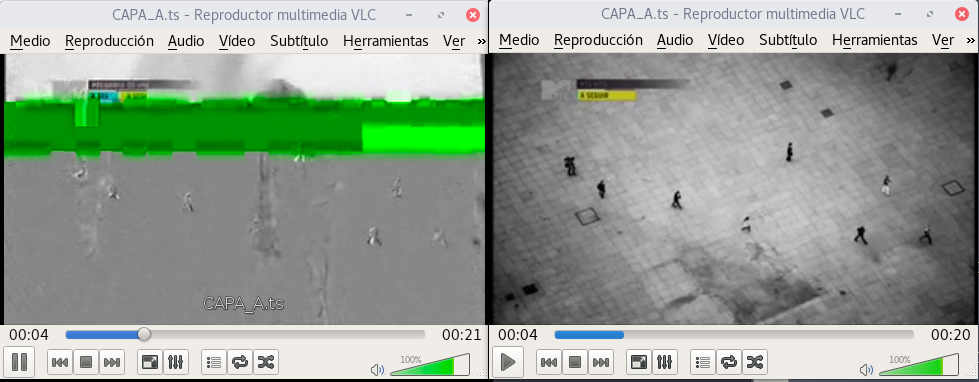
\includegraphics[scale=0.35]{calidad_imagen}
		%\caption{Umbral de ruido encontrado en ambiente controlado}
	\end{figure}
\end{frame}

%\subsection{Pruebas en canal real}

\begin{frame}{Pruebas en canal real}
\begin{block}{Pruebas contra gr-isdbt en otra PC}
	\begin{itemize}	
		\item { Encontramos  }
		\item { Verificamos la funcionalidad basica del sistema }
	\end{itemize}
\end{block}

\begin{block}{Pruebas contra equipo comercial Rohde-Schwarz}
\begin{columns}
	\column{0.5\textwidth}
	\begin{itemize}	
		\item {	Observamos la constelación recibida, detectamos un bug importante }
		\item { Primeras diferencias notorias entre gr-isdbt-Tx y los transmisores comerciales }
	\end{itemize}
	\column{0.5\textwidth}
	\begin{figure}
		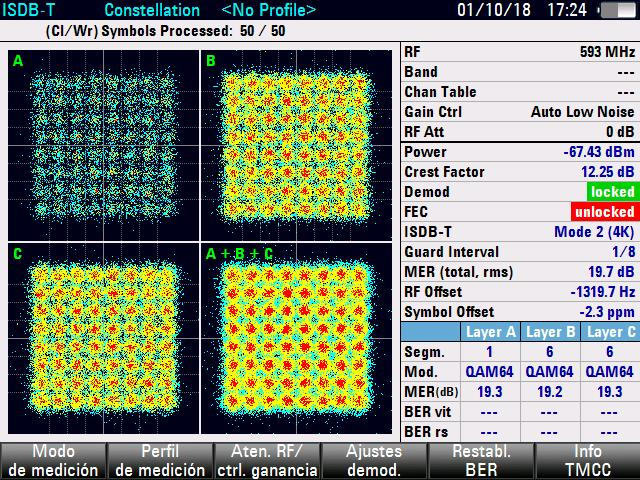
\includegraphics[scale=0.25]{constelacion_eth}
		%\caption{Señal recibida en un analizador de TV}
	\end{figure}
\end{columns}
\end{block}
\end{frame}

\begin{frame}{Pruebas en canal real}
\begin{block}{Pruebas contra televisor comercial}
	\begin{itemize}	
		\item { Comprobamos que funcionan las tres capas correctamente  }
		\item { Se cumple con los objetivos planteados al principio del proyecto }
	\end{itemize}
\end{block}

	\begin{figure}
	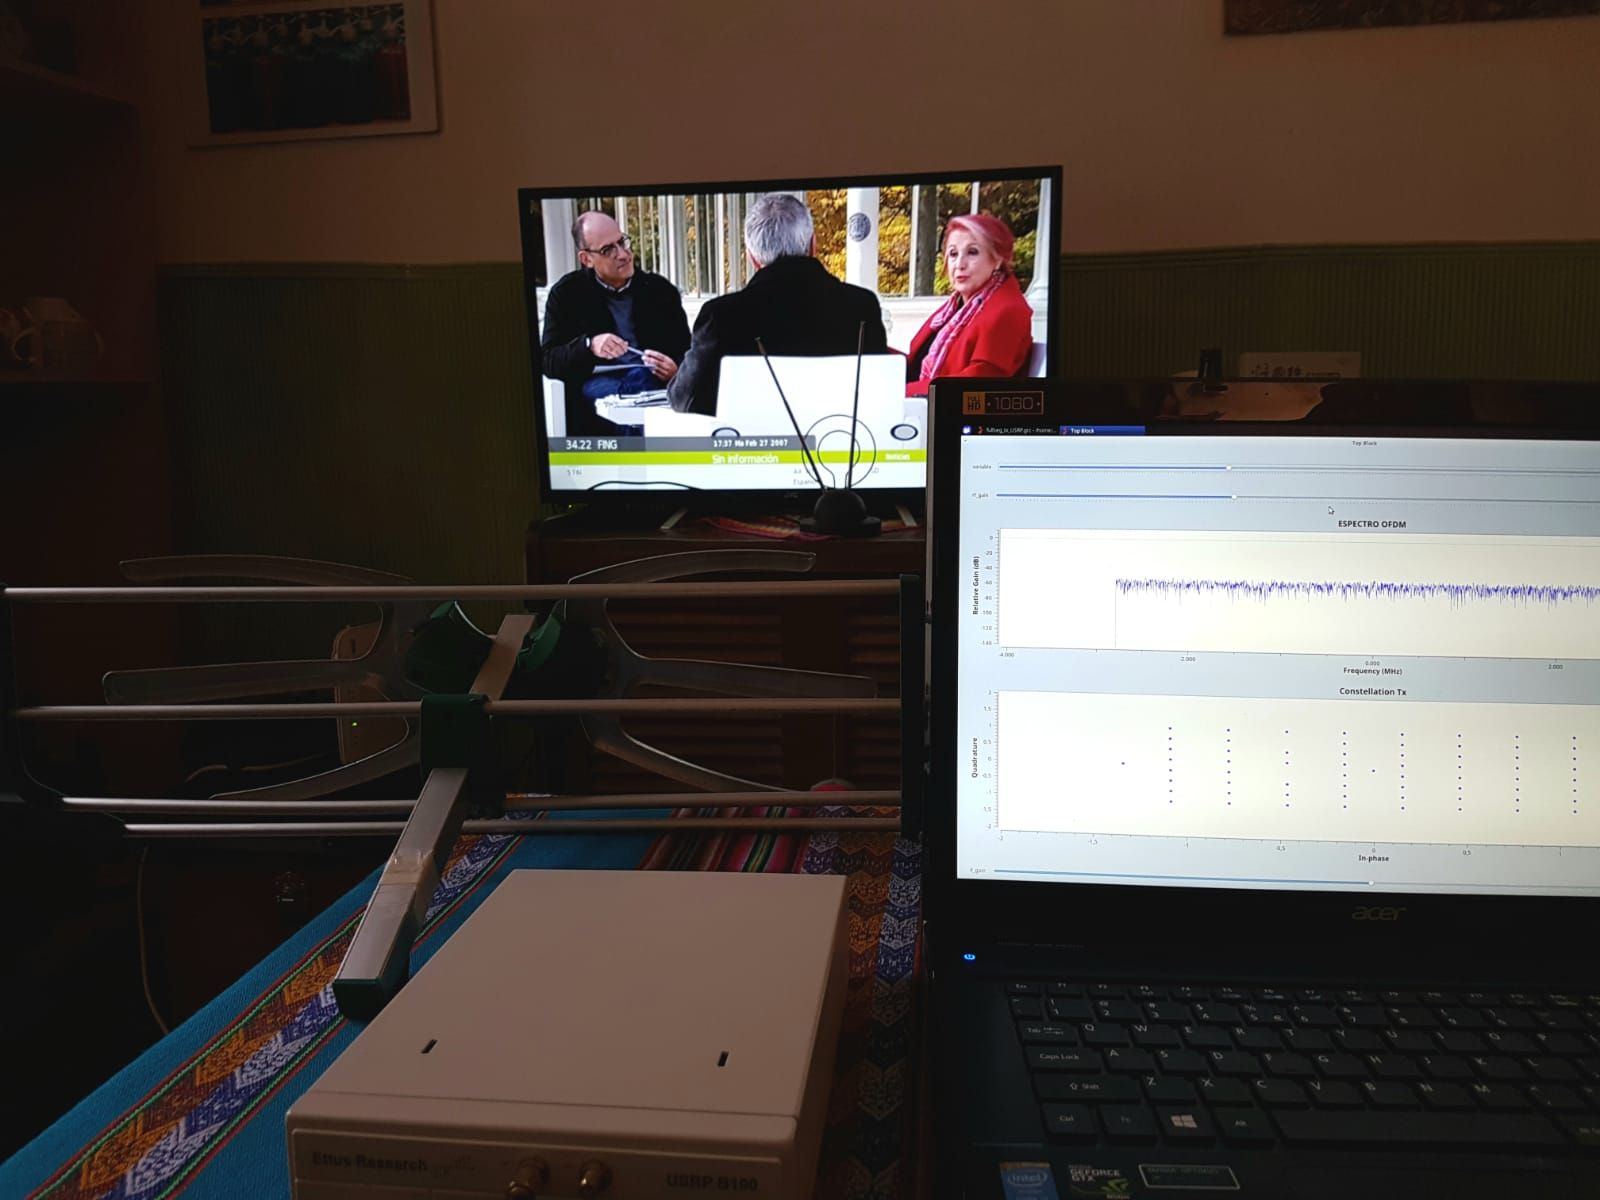
\includegraphics[scale=0.11]{contra_tele}
	%\caption{Sistema gr-isdbt-Tx en funcionamiento}
	\end{figure}

\end{frame}